\section{Tugas 2 -- Prediksi Sisa Umur Pakai (RUL)}
Data latih: \TduaNUnitTrain{} mesin dengan riwayat sampai rusak (median umur \TduaUmurMedian{} siklus); data uji \TduaNUnitTest{} mesin yang dipotong pada titik acak
(panjang \TduaUjiMin--\TduaUjiMaks{} siklus, median \TduaUjiMedian). RUL diprediksi di siklus terakhir tiap mesin uji.

\subsection*{(a) Eksplorasi dan preprocessing}
Tiga setelan operasi membentuk enam kondisi diskrit (Tabel~\ref{tab:t2_kondisi}). Bacaan sensor terutama ditentukan oleh kondisi operasi, sehingga tren degradasi
baru terlihat setelah setiap sensor di-z-score \emph{per kondisi} (Gambar~\ref{fig:t2kondisi}); normalisasi global akan menyamarkan tren dengan lompatan antar kondisi.
Statistik normalisasi dihitung hanya dari unit latih pada setiap fold. Bacaan hilang (\TduaNaNPersen\%) diisi dengan nilai sebelumnya dalam unit yang sama
(\emph{forward-fill}, kausal). \emph{Spike} ($|z| > 6$, \TduaSpike{} titik) diganti nilai sebelumnya. Sensor dengan |korelasi Spearman| dengan RUL < 0,05 dibuang
(\TduaSensorDibuang; Tabel~\ref{tab:t2_sensor}), menyisakan \TduaSensorDipakai{} sensor ditambah one-hot kondisi dan nomor siklus.

\begin{figure}[ht]\centering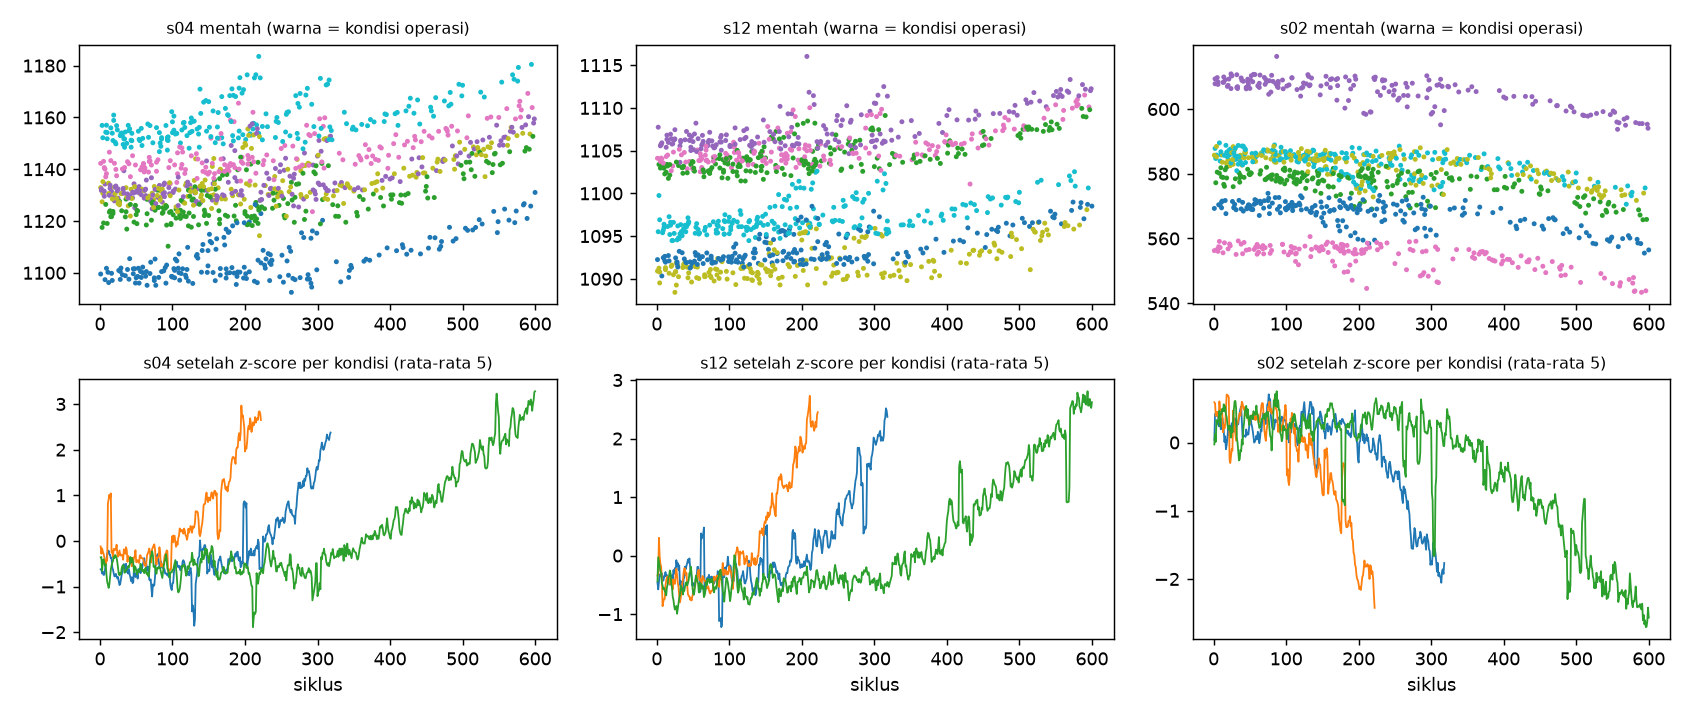
\includegraphics[width=\linewidth]{t2_eda_kondisi.png}
\caption{Atas: sensor mentah (warna = kondisi operasi). Bawah: setelah z-score per kondisi, tren degradasi terlihat.}\label{fig:t2kondisi}\end{figure}
\begin{table}[ht]
\centering\small
\resizebox{\ifdim\width>\linewidth\linewidth\else\width\fi}{!}{%
\begin{tabular}{rrrrr}
\toprule
kondisi & setel\_1 & setel\_2 & setel\_3 & n\_baris \\
\midrule
0 & 20.000 & 0.700 & 100.000 & 42600 \\
1 & 10.000 & 0.250 & 100.000 & 42078 \\
2 & 25.000 & 0.620 & 60.000 & 42211 \\
3 & 42.000 & 0.840 & 100.000 & 42640 \\
4 & 0.000 & -0.000 & 100.000 & 42393 \\
5 & 35.000 & 0.840 & 100.000 & 42252 \\
\bottomrule
\end{tabular}
}
\caption{Enam kondisi operasi hasil clustering setelan (median setelan per kondisi).}
\label{tab:t2_kondisi}
\end{table}

\begin{table}[ht]
\centering\small
\resizebox{\ifdim\width>\linewidth\linewidth\else\width\fi}{!}{%
\begin{tabular}{lrrr}
\toprule
sensor & std\_maks\_per\_kondisi & spearman\_rul & dipakai \\
\midrule
s04 & 8.147 & -0.741 & True \\
s12 & 2.161 & -0.435 & True \\
s15 & 6.544 & -0.430 & True \\
s08 & 4.181 & -0.277 & True \\
s09 & 7.499 & -0.243 & True \\
s18 & 7.922 & -0.001 & False \\
s05 & 2.854 & -0.001 & False \\
s01 & 6.355 & 0.000 & False \\
s16 & 8.082 & 0.001 & False \\
s06 & 4.867 & 0.003 & False \\
s19 & 6.686 & 0.003 & False \\
s10 & 4.538 & 0.003 & False \\
s11 & 13.094 & 0.175 & True \\
s21 & 9.501 & 0.214 & True \\
s20 & 15.333 & 0.235 & True \\
s14 & 7.550 & 0.246 & True \\
s13 & 10.630 & 0.248 & True \\
s17 & 4.181 & 0.253 & True \\
s03 & 9.489 & 0.414 & True \\
s07 & 4.989 & 0.415 & True \\
s02 & 5.481 & 0.425 & True \\
\bottomrule
\end{tabular}
}
\caption{Skor sensor: std maksimum per kondisi dan korelasi Spearman dengan RUL (setelah normalisasi).}
\label{tab:t2_sensor}
\end{table}


\subsection*{(b) Label}
Untuk setiap mesin latih, $\mathrm{RUL}_t = \text{siklus terakhir} - t$, lalu dipotong pada 150 (Gambar~\ref{fig:t2label}): di awal umur mesin, degradasi belum terlihat
sehingga RUL besar tidak dapat dibedakan; pemotongan juga sesuai definisi label uji.

\begin{figure}[ht]\centering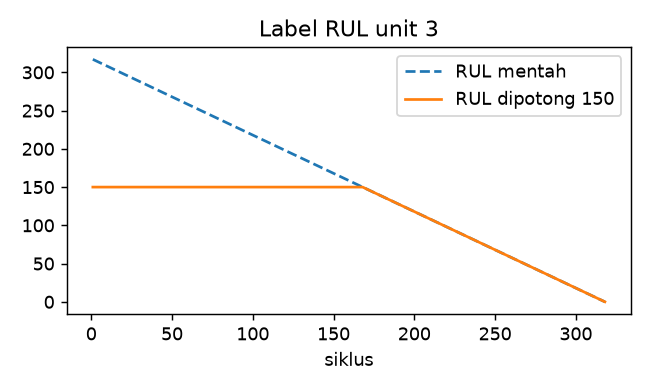
\includegraphics[width=.45\linewidth]{t2_label.png}
\caption{Label RUL mentah dan setelah dipotong 150.}\label{fig:t2label}\end{figure}

\subsection*{(c) Sekuens tanpa kebocoran}
Setiap sampel adalah jendela 40 siklus yang \emph{berakhir} di siklus $t$, dengan target RUL di $t$. Semua mesin disusun dengan padding nol di kiri ditambah kanal mask,
sehingga histori yang lebih pendek dari 40 siklus tetap dapat diproses dan jendela tidak pernah berisi siklus sesudah $t$ atau siklus mesin lain
(diuji otomatis di \texttt{kode/tests/test\_rul\_windows.py}).

\subsection*{(d)--(e) Model dan validasi per mesin}
Dibandingkan GRU dua lapis, TCN (konvolusi kausal berdilatasi 1--8), GRU dengan loss asimetris (kesalahan terlalu optimis diberi bobot 1,6), dan baseline non-DL LightGBM
pada fitur jendela (nilai terakhir, rata-rata 10 siklus, kemiringan 20 siklus). Validasi 3-fold \emph{per mesin} (GroupKFold); setiap mesin validasi dipotong pada tiga
titik acak (panjang $\geq 50$ siklus) seperti data uji, lalu RUL dievaluasi hanya di siklus terakhir yang terlihat --- mengevaluasi semua jendela akan terlalu optimis.
RMSE: GRU \TduaRMSEGRU, TCN \TduaRMSETCN, GRU loss asimetris \TduaRMSEAsim, LightGBM \TduaRMSELGBM; skor asimetris per 300 mesin: \TduaSkorGRU, \TduaSkorTCN, \TduaSkorAsim, \TduaSkorLGBM
(Tabel~\ref{tab:t2_model}--\ref{tab:t2_skor_rentang}). Terpilih \textbf{\TduaKonfigArsitektur}.
Karena skor menghukum prediksi terlambat lebih berat, prediksi digeser $\delta = \TduaKonfigBias$ siklus (dipilih pada prediksi out-of-fold), mengubah skor dari
\TduaSkorSebelumBias{} menjadi \TduaSkorSesudahBias{} dengan RMSE \TduaRMSESesudahBias{} (Gambar~\ref{fig:t2bias}).
Error terbesar ada pada rentang RUL 50--100 (RMSE TCN 29.7, dibanding 12.0 pada RUL 0--25), dan rentang ini juga menyumbang sebagian besar skor asimetris. Pada fase ini degradasi baru mulai sehingga sinyal sensor belum jelas berubah, sedangkan mendekati kerusakan (RUL $<$ 25) tren sensor sudah tegas dan prediksi jauh lebih akurat. Koreksi bias $\delta = -14$ sengaja menaikkan RMSE (20.52 $\to$ 22.85) demi menurunkan skor asimetris hampir separuhnya, karena prediksi yang terlambat jauh lebih mahal daripada yang terlalu dini.
\begin{table}[ht]
\centering\small
\resizebox{\ifdim\width>\linewidth\linewidth\else\width\fi}{!}{%
\begin{tabular}{lrrrrrr}
\toprule
model & rmse & skor\_asimetris\_per\_300\_unit & rmse\_rul\_0\_25 & rmse\_rul\_25\_50 & rmse\_rul\_50\_100 & rmse\_rul\_100\_150 \\
\midrule
TCN (1D-CNN dilatasi) & 20.524 & 6905.118 & 11.988 & 17.677 & 29.691 & 17.000 \\
LightGBM (baseline non-DL) & 20.874 & 7072.671 & 10.927 & 17.727 & 30.636 & 17.175 \\
GRU & 24.416 & 23278.234 & 12.257 & 19.977 & 34.311 & 21.570 \\
GRU + loss asimetris & 24.566 & 20430.217 & 11.035 & 20.502 & 33.458 & 22.566 \\
\bottomrule
\end{tabular}
}
\caption{Perbandingan model (3-fold per mesin, evaluasi di titik potong acak seperti data uji).}
\label{tab:t2_model}
\end{table}

\begin{table}[ht]
\centering\small
\resizebox{\ifdim\width>\linewidth\linewidth\else\width\fi}{!}{%
\begin{tabular}{lrrrr}
\toprule
model & skor\_rul\_0\_25 & skor\_rul\_25\_50 & skor\_rul\_50\_100 & skor\_rul\_100\_150 \\
\midrule
TCN (1D-CNN dilatasi) & 783.576 & 7513.533 & 20794.864 & 1490.349 \\
LightGBM (baseline non-DL) & 689.235 & 7136.239 & 21308.650 & 1677.989 \\
GRU & 865.379 & 59792.506 & 58087.709 & 3257.132 \\
GRU + loss asimetris & 754.139 & 51706.650 & 49658.233 & 3676.140 \\
\bottomrule
\end{tabular}
}
\caption{Skor asimetris per rentang RUL aktual (dinormalisasi per 300 unit).}
\label{tab:t2_skor_rentang}
\end{table}

\begin{figure}[ht]\centering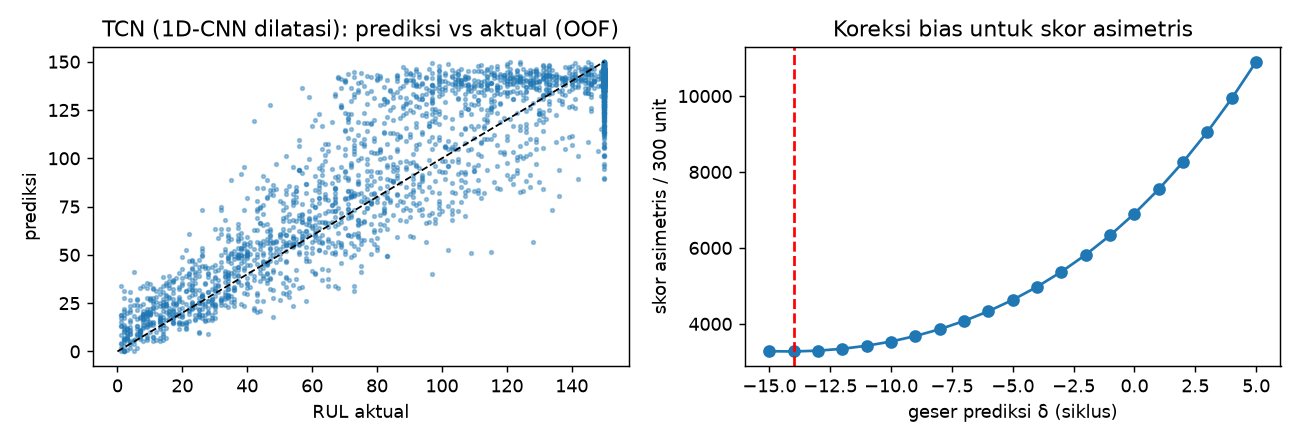
\includegraphics[width=.9\linewidth]{t2_prediksi_bias.png}
\caption{Kiri: prediksi out-of-fold vs aktual. Kanan: pemilihan pergeseran $\delta$ untuk skor asimetris.}\label{fig:t2bias}\end{figure}
\begin{figure}[ht]\centering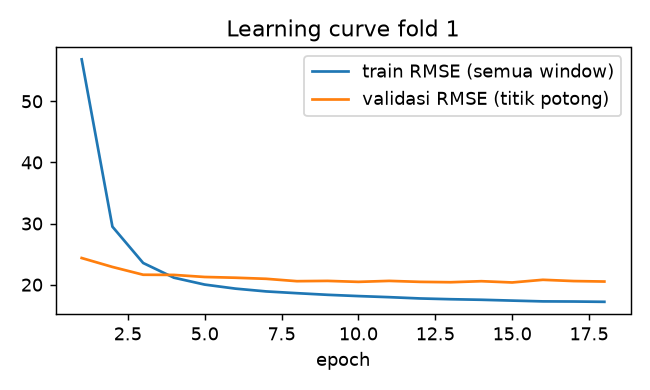
\includegraphics[width=.55\linewidth]{t2_learning_curve.png}
\caption{Learning curve model terpilih pada fold 1: RMSE latih vs RMSE validasi di titik potong.}\label{fig:t2lc}\end{figure}
Gambar~\ref{fig:t2lc} membandingkan RMSE latih (rata-rata semua window) dengan RMSE validasi yang diukur hanya di titik potong seperti data uji. RMSE validasi wajar lebih tinggi karena titik potong lebih sulit diprediksi daripada rata-rata window. Model dilatih dengan jumlah epoch tetap tanpa \emph{early stopping}; sebagai gantinya, risiko overfit diredam dengan dropout, \emph{weight decay}, dan rata-rata tiga seed pada model final. Selisih antara kedua kurva di epoch akhir menunjukkan seberapa besar model mulai menghafal pola data latih.
\subsection*{(f) Ketidakpastian dan kapan servis}
Interval prediksi dibuat dengan MC dropout (30 kali forward dengan dropout aktif pada GRU). Interval 80\% mencakup RUL aktual pada \TduaCoverageInterval{} sampel
validasi dengan lebar median \TduaLebarInterval{} siklus (Gambar~\ref{fig:t2interval}). Kebijakan servis yang diusulkan memakai \emph{batas bawah} interval:
servis bila batas bawah $\leq H$ siklus. Tabel~\ref{tab:t2_kebijakan_servis} menunjukkan trade-off antara mesin hampir rusak yang tertangkap dan servis yang terlalu dini;
dengan $H = 20$, \TduaUjiServis\% mesin uji direkomendasikan diservis.
Kami memilih $H = 30$. Pada validasi, aturan ini menangkap 96.7\% mesin yang benar-benar hampir rusak (RUL $\leq 15$) tanpa satu pun servis yang terlalu dini (RUL $> 80$), dengan 16.0\% mesin diservis; menaikkan $H$ ke 40 hanya menambah tangkapan 3.3 poin tetapi menambah servis. Alasannya, biaya mesin rusak saat produksi (berhenti mendadak dan kerusakan lanjutan) jauh lebih besar daripada biaya satu servis yang agak terlalu awal. Dengan $H = 30$, 23.0\% mesin uji direkomendasikan diservis. Catatan: interval MC dropout terlalu sempit (coverage hanya 0.338 dari target 0.80), sehingga kebijakan ini kami dasarkan pada hasil empiris di validasi, bukan pada nominal 80\%-nya.
\begin{figure}[ht]\centering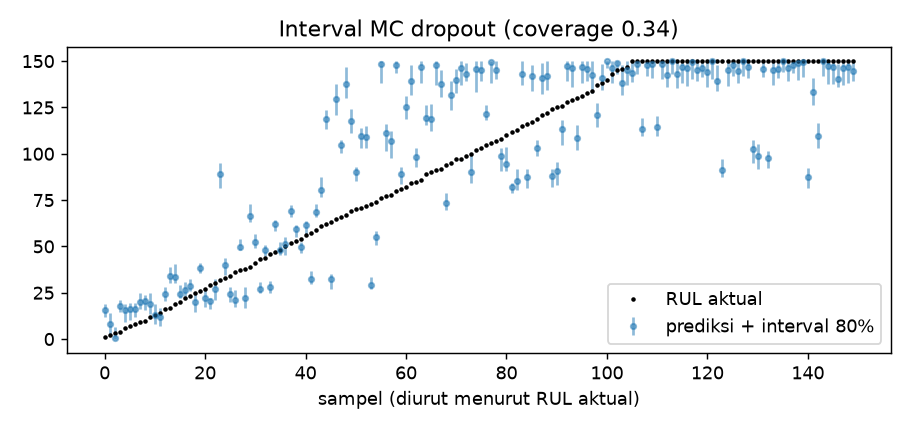
\includegraphics[width=.7\linewidth]{t2_interval.png}
\caption{Prediksi dan interval 80\% MC dropout pada sampel validasi (diurutkan menurut RUL aktual).}\label{fig:t2interval}\end{figure}
\begin{table}[ht]
\centering\small
\resizebox{\ifdim\width>\linewidth\linewidth\else\width\fi}{!}{%
\begin{tabular}{rrrr}
\toprule
H (servis bila batas bawah $\leq$ H) & mesin diservis (\%) & tertangkap, RUL $\leq$ 15 (\%) & terlalu dini, RUL > 80 (\%) \\
\midrule
10 & 5.1 & 51.4 & 0.0 \\
20 & 11.5 & 86.8 & 0.0 \\
30 & 16.0 & 96.7 & 0.0 \\
40 & 20.4 & 100.0 & 0.2 \\
50 & 24.9 & 100.0 & 0.4 \\
\bottomrule
\end{tabular}
}
\caption{Kebijakan servis berbasis batas bawah interval 80\% (MC dropout, GRU, OOF).}
\label{tab:t2_kebijakan_servis}
\end{table}


\textbf{Prediksi uji.} Model terpilih dilatih ulang pada semua mesin latih dengan tiga seed (ensemble), lalu digeser $\delta$ dan dipotong ke $[0,150]$;
median RUL uji \TduaUjiMedianRUL{} siklus. Interval per mesin disimpan di \texttt{kode/outputs/tables/t2\_interval\_uji.csv}.
